\section{Security and Privacy Analysis}
\label{sec:analysis}
In this section, we analyze the security and privacy guarantees provided by UPPRESSO and show that it achieves all four required security properties defined in Section~\ref{subsec:basicrequirements} and prevents both types of privacy threats against SSO services.

%\subsection{Extended Adversarial Models}
\label{adver-model}
\textcolor{blue}{Threat model defined in Section~\ref{subsec:threatmodel} depicts potential adversaries against SSO as honest-but-curious IdPs, malicious RPs, and malicious users, where malicious RPs and users could collude. Based on their objectives, we consider three adversarial scenarios in the security analysis and present our goals in each scenario: {\bf \emph{(S1)}} malicious users colluding with each other or with malicious RPs to impersonate an honest user and log in to an honest RP, which requires satisfying {\em four SSO security properties}; {\bf \emph{(S2)}} the honest-but-curious IdP inferring the identity of the RP(s) that the user requests to access, which requires {\em privacy against the IdP}; and {\bf \emph{(S3)}} malicious RPs colluding with each other or with malicious users to deduce the user identity or link her pseudo-identities, which requires {\em privacy against colluding RPs}. Next, we prove that UPPRESSO is secure in the first adversarial scenario in Section~\ref{analysis-security} and it can prevent privacy threats in the other two adversarial scenarios in Section~\ref{sec-:analysis}.}

%======move to security analysis
%The RP cannot derive $ID_U$ from either $PID_U$ or $Acct$ due to the elliptic curve discrete logarithm problem (ECDLP). Since $t$ is random in $\mathbb{Z}_n$ and unknown to the IdP, from the IdP's view, $PID_{RP}$ is indistinguishable from a random variable on $\mathbb{E}$. So, the IdP cannot learn anything about $ID_{RP}$ from $PID_{RP}$. 
%Section \ref{sec:analysis} presents more detailed analyses.

\subsection{Security}
\label{analysis-security}
%UPPRESSO satisfies four sufficient conditions (i.e., RP designation, user identification, integrity, and confidentiality of identity tokens) of secure SSO services \cite{ArmandoCCCT08,FettKS16, FettKS17}, as stated in Section \ref{subsec:basicrequirements}.

\textcolor{blue}{In a secure SSO service that is robust against impersonation attacks, an honest user should be able to prove her identity to the target RP with an identity token issued by the IdP. As pseudo-identities are used in UPPRESSO, it is important to allow the RP to verify that ({\em a}) $PID_{RP}$ included in the identity token is a transformation from its $ID_{RP}$ and tied to the current login instance, which requires {\em RP designation}; and ({\em b}) $PID_U$ included in the identity token maps to a unique, long-term user account, which requires {\em user identification}. Besides, the identity token for an honest RP should not be intercepted by malicious users or RPs, requiring the {\em confidentiality of identity tokens}, nor be forged or tampered with to include a fake $PID_U$ or $PID_{RP}$, requiring the {\em integrity of identity tokens}.}

To prove that UPPRESSO satisfies these four properties, we first formalize its login flow using a Dolev-Yao-style model \cite{SPRESSO}, % which has been used in the formal analysis of SSO protocols such as OAuth 2.0 \cite{FettKS16} and OIDC \cite{FettKS17}.
which abstracts the entities in a web system, such as web servers and browsers, as \emph{atomic processes} %which communicate with each other through events. % such as HTTPS request and response.
and then defines \emph{script processes} to formulate client-side scripts.
%The script is dependently invoked by the browser to process the server-defined logic.%such as verifying $Certificate_{RP}$. %postmessage events; %atomic process <-> script process, communication. %Other events change self-trigger. 
Therefore, the atomic processes of UPPRESSO include an {\em IdP process}, a finite set of {\em web servers} for honest RPs, a finite set of honest {\em browsers}, and a finite set of {\em attacker processes} that model malicious RPs and malicious users. The processes communicate with each other through events such as HTTPS requests and responses. A browser may have an honest IdP script and multiple RP scripts that could be honest or malicious.
%Although the scripts coexist in the same browser, they are strictly separated.
The script processes communicate with each other through \verb+postMessage+, which are modeled as transmitted-to-itself events of a browser process.
%To clearly indicate the action of postMessage communication, we define it as the transmitting-to-itself event of the browser (which is not defined in SPRESSO).

\textcolor{blue}{With this formal model, we could (\emph{a}) trace the identity token lifecycle from its generation at the IdP to its acceptance at the RP to prove that it cannot be leaked to adversaries; (\emph{b}) locate the places where $PID_U$, $PID_{RP}$, and other elements in the identity token are processed to prove that they cannot be manipulated by any adversary; and (\emph{c}) locate the places where the IdP script uses $PK$ for verification to prove that it cannot be replaced by any adversary. Besides, we show that the IdP cannot view $t$ shared only between the user and the RP, while the RPs cannot view $u$ shared between the user and the IdP. It is trivial to prove the security of $r$, as it never leaves the IdP.
%These conclusions are used to prove the security of the UPPRESSO protocols.
}

\vspace{1mm}
\noindent\textcolor{blue}{\textbf{RP Designation.}~~Provided that $r$ is known to only the IdP,
the RP pseudo-identity $PID_{RP}$ in the identity token
     designates the target RP with $ID_{RP} = [r]G$, and only this RP.}

\vspace{0.75mm}
\noindent\textbf{Proof.}
\textcolor{blue}{As analyzed in the Dolev-Yao style model, $PID_{RP} = [t]ID_{RP}$
        is set by the honest IdP and no adversaries manipulate it.}
Then, $PID_{RP} = [t]ID_{RP}$ in the the identity token is expected by the target RP,
    because $t$ is also sent to this RP with $ID_{RP}$
     and this RP checks that $PID_{RP}$ is equal to $[t]ID_{RP}$.
So $PID_{RP}$ designates this RP.


Based on the ECDLP
    we prove that,
    for adversaries,
        the probability of finding $t$ and $t'$
    satisfying $[t]ID_{RP_j} = [t']ID_{RP_{j'}}$ is negligible,
    where $RP_j$ and $RP_{j'}$ are any two RPs in the finite set of RPs (i.e.,
    $ID_{RP_j} = [r_j]G$ and $ID_{RP_{j'}} = [r_{j'}]G$, while $r_j$ and $r_{j'}$ are kept secret to the adversaries).
This negligible probability means $PID_{RP_j} = [t]ID_{RP_j}$ designates \emph{only} the target RP with $ID_{RP_j}$.

Let $\mathbb{E}$ be an elliptic curve, %over a finite field $\mathbb{F}_q$,
    $G$ be a point on $\mathbb{E}$ of order $n$,
        and $Q = [x]G$ where $x$ is a random integer in $\mathbb{Z}_n$.
Given $G$ and $Q$,
    the probability that a probabilistic polynomial time (PPT) algorithm calculates $x$ (i.e., solves the ECDLP) is negligible.
For any PPT algorithm $\mathcal{D}$ to calculate $x$, we define
\begin{equation*}
{\rm Pr}\{\mathcal{D}(G, [x]G)=x\} = \epsilon_{c}(k)
\end{equation*}
Here, ${\rm Pr}\{\}$ denotes the probability.
So $\epsilon_{c}(k)$ becomes negligible with the increasing security parameter $k$.

Assume a game $\mathcal{G}_c$ between an adversary and a challenger,
    to describe this $PID_{RP}$-collision attack:
the adversary receives a finite set of RP identities from the challenger,
 denoted as ($ID_{RP_1}$, $ID_{RP_2}$, ..., $ID_{RP_m}$)
 where $m$ is the amount of all RPs in the system,
  and then outputs $(a, b, t, t')$.
If $[t]ID_{RP_a}=[t']ID_{RP_b}$, the adversary succeeds in this game.
%If the adversary has the non-negligible probability on succeeding in this game, RP designation is broken.
Note that $m$ is a finite integer, and $m \ll 2^k$ as $k$ increases.
We define the probability that the adversary succeeds in this game as ${\rm Pr}_s$.


\begin{figure}[tb]
  \centering
  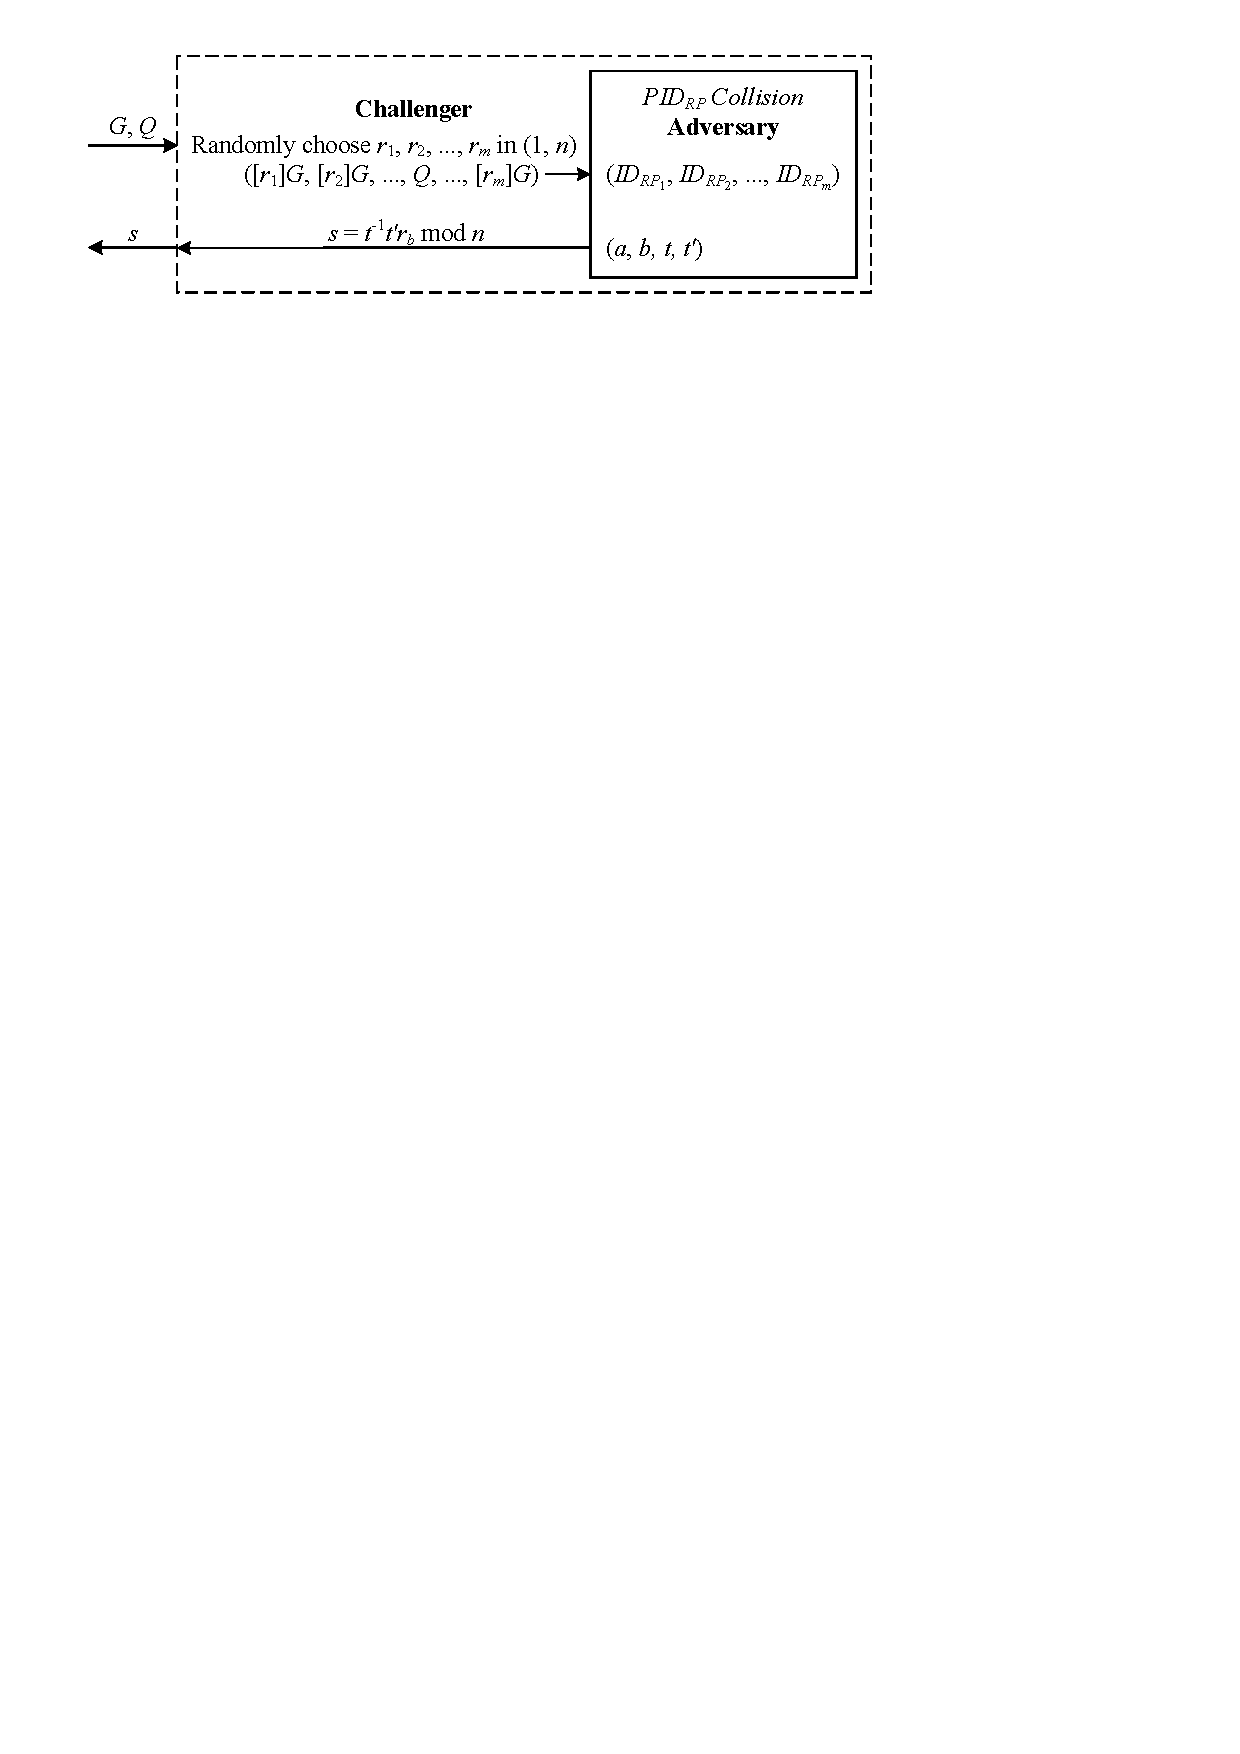
\includegraphics[width=0.97\linewidth]{fig/ecdlp_algorithm.pdf}
  \caption{The algorithm based on the $PID_{RP}$ collision, to solve the ECDLP}
  \label{fig:ecdlp_algorithm}
\end{figure}


Figure \ref{fig:ecdlp_algorithm} shows a PPT algorithm $\mathcal{D}^*_c$ based on this game, to solve the ECDLP.
The input of $\mathcal{D}^*_c$ is in the form of ($G$, $Q$).
On receiving an input, the challenger of $\mathcal{G}_c$ randomly chooses $r_1, r_2, \cdots, r_m$ in $\mathbb{Z}_n$,
 calculates $[r_1]G, [r_2]G, \cdots, [r_m]G$,
 and randomly replaces some $[r_j]G$ with $Q$.
Then,
    these $m$ RP identities are sent to the adversary,
which returns the result ($a$, $b$, $t$, $t'$).
Finally, the challenger of $\mathcal{G}_c$ calculates $s = t^{-1}t'r_b \bmod n$ and returns $s$ as the output of $\mathcal{D}^*_c$.

If $[r_a]G$ happens to be replaced with $Q$ and the adversary of $\mathcal{G}_c$ succeeds,
    we find $Q = [s]G$ and then $s=x$ because $[tr_a]G = [t]Q = [t'r_b]G$.
As $[r_j]G$ is randomly replaced by the challenger,
    $Q$ and other RP identities in the input set are indistinguishable to the adversary.
Thus,
\begin{equation*}
{\rm Pr}\{\mathcal{D}^*_c(G, [x]G)=x\} = {\rm Pr}\{s = x\}={\rm Pr}\{a=j\}{\rm Pr}_s=\frac{1}{m}{\rm Pr}_s
\end{equation*}

If the adversary is able to find $t$ and $t'$
    satisfying that $[t]ID_{RP_j} = [t']ID_{RP_{j'}}$,
    it will have advantages in $\mathcal{G}_c$
        and then
         ${\rm Pr}_s$ becomes non-negligible as $k$ increases.
Because $m$ is a finite integer, ${\rm Pr}\{\mathcal{D}^*_c(G, [x]G)=x\} = \frac{1}{m}{\rm Pr}_s$ also
becomes non-negligible with the increasing $k$.
This violates the ECDLP assumption.
Thus, the probability of finding $t$ and $t'$ satisfying that $[t]ID_{RP_j} = [t']ID_{RP_{j'}}$ in UPPRESSO is negligible,
    so this token binding $PID_{RP}$
     is expected by \emph{only} the target RP.
$\square$


\vspace{1mm}
\noindent\textcolor{blue}{\textbf{User Identification.}~~In the identity token
    binding $PID_U$ and $PID_{RP}$,
the user pseudo-identity $PID_U$ identifies
        the authenticated user with $ID_U$, % as $Acct = [ID_U][ID_{RP}]$,
         and only this user,  at the target RP with $ID_{RP} = [r]G$.}
%That is,
%in UPPRESSO, $Acct$ identifies the mapping $[ID_u][ID_{RP}]$.

\vspace{0.75mm}
\noindent\textbf{Proof.}
$PID_U$ in identity token identifies the authenticated user as $Acct = [ID_U]ID_{RP}$
    at the RP with $ID_{RP}$ as follows.
\textcolor{blue}{$PID_U = [ID_U]PID_{RP}$ is calculated by the IdP based on the user authenticated as $ID_U = u$,
    which is analyzed in the Dolev-Yao style model.}
In the meantime, the  RP checks that $PID_{RP} = [t]ID_{RP}$
    and calculates $Acct = [t^{-1}]PID_U = [t^{-1}][ID_U]PID_{RP} = [t^{-1}][ID_U][t]ID_{RP} = [ID_U]ID_{RP}$.
%$t$ and $PID_{RP}$ have been checked by the honest RP in the $PID_{RP}$-registration result,
Thus, given a user with $ID_U$, an RP with $ID_{RP}$ always derives an identical account
 $[ID_U]ID_{RP}$ from different identity tokens. % binding $PID_U$ and $PID_{RP}$.
%because in the user's any $i$-th and $i'$-th ($i \neq i'$) login instances to the RP,
% $\mathcal{F}_{Acct}(PID_{U}^i, PID_{RP}^i) = \mathcal{F}_{Acct}(PID_{U}^{i'}, PID_{RP}^{i'}) = [ID_U]ID_{RP}$.

$Acct =  [ID_U]ID_{RP}$ identifies \emph{only} this user.
$\mathbb{E}$ is a finite cyclic group,
    and then $ID_{RP} = [r]G$ is also a generator of order $n$.
Thus, given any RP,
    $[u]ID_{RP}$ assigns a \emph{unique} account to the user,
        because $1 \leq u < n$ and $ID_U = u$ is unique. $\square$


%The detailed process of proof is shown in Appendix.
\vspace{1mm}
\noindent\textcolor{blue}{\textbf{Integrity.}~~An honest RP accepts only identity tokens
 binding its pseudo-identity $PID_{RP}$ and the authenticated user's pseudo-identity $PID_U$,
 and actually binding $ID_{RP}$ and $Acct=[ID_U]ID_{RP}$,
 when $SK$ is held by only the IdP.}

\vspace{0.75mm}
\noindent\textbf{Proof.}
A signed identity token binds $PID_{RP} = [t]ID_{RP}$ and $PID_U = [ID_U]PID_{RP}$,
    % $Acct$ and $ID_{RP}$ implicitly,
    and any breaking results in some failed checking or verification in the login flow as below.
%It is ensured by the IdP's signatures:
First of all, the identity token is signed by the honest IdP using $SK$
        and verified by the RP using $PK$,
        so any modification will be rejected by the RP.
According to the proof of RP designation,
   % there is no $t' \neq t$ but satisfying that $PID_{RP} = [t]ID_{RP_j} = [t']ID_{RP_{j'}}$.
   $PID_{RP}$ identifies only the RP with $ID_{RP}$;
   according to the proof of user identification,
    $PID_U$ identifiers only the user with $Acct = [ID_U]ID_{RP}$ at the RP.
Therefore, the identity token explicitly binding $PID_U$ and $PID_{RP}$,
    matches \emph{only} one $ID_{RP}$ and \emph{only} one $Acct = [t^{-1}]PID_{U}$.
Therefore,
    $Acct$ and $ID_{RP}$ are actually bound in the token by the IdP's signatures,
        due to the one-to-one mapping between (\emph{a}) the pair of $Acct$ and $ID_{RP}$ and (\emph{b}) the triad of $PID_U$, $PID_{RP}$, and $t$. $\square$


\vspace{1mm}
\noindent\textcolor{blue}{\textbf{Confidentiality.}~~An identity token
    is accessible to only
                the authenticated user and the target RP, in addition to the IdP signing this token.}

\vspace{0.75mm}
\noindent\textbf{Proof.}
\textcolor{blue}{As analyzed in the Dolev-Yao style model, no event leaks an identity token to any malicious entity other than the authenticated user and the designated RP.}
First of all, the communications among the IdP, RPs and users,
    are protected by HTTPS,
    and the \verb+postMessage+ HTML5 API ensures the dedicated channels between two scripts within the browser,
    so no other entities can eavesdrop the identity tokens.
Further, the IdP sends an identity token only to the authenticated user
        (i.e., the IdP script).
The IdP script forwards the token to the RP script
 only if it is downloaded from the same origin as $Enpt_{RP}$,
while the binding of $Enpt_{RP}$ and $ID_{RP}$ is ensured by a verified RP certificate
    and $PK$ is well set in the honest IdP script.
  %  which is verified by the IdP script.
So only the RP that owns $Enpt_{RP}$ and $ID_{RP}$,
    receives this token. $\square$



\subsection{Privacy}
\label{sec-:analysis}
UPPRESSO effectively prevents the privacy threats of IdP-based login tracing and RP-based identity linkage.

\textcolor{blue}{The information accessible to the IdP and derived from the RP's identity,
    is only $PID_{RP}$ in identity-token requests, where $PID_{RP} = [t]ID_{RP}$ is calculated by a user.
    % and $t$ is kept secret to the IdP.
So the prevention against the IdP-based login tracing in UPPRESSO
    is expressed formally as below.}

\vspace{1mm}
\noindent\textcolor{blue}{\textbf{Privacy against the IdP.}~~If $t$ is random in $\mathbb{Z}_n$ and unknown to the IdP,
the IdP
 cannot infer any information about $ID_{RP_j}$ or link any pair of $PID_{RP_j}^i$ and $PID_{RP_{j'}}^{i'}$
  ($i \neq i'$ but $j = j'$),
    from a user's identity-token requests for $PID_{RP_j}^i$ ($i,j = 1, 2, \cdots$).}

\vspace{0.75mm}
\noindent\textbf{Proof.}
Because (\emph{a}) $ID_{RP} = [r]G$ is also a generator of order $n$,
        where $G$ is a generator of finite cyclic group $\mathbb{E}$,
    \textcolor{blue}{and (\emph{b}) $t$ is a random number in $\mathbb{Z}_n$ and kept unknown to the IdP,}
 from the IdP's view,
 $PID_{RP}$
is \emph{indistinguishable} from a random variable on $\mathbb{E}$.
Thus,
    the IdP cannot infer any information about $ID_{RP}$ from $PID_{RP} = [t]ID_{RP}$,
or distinguish $[t]ID_{RP_j} = [tr]G$ from any other $[t']ID_{RP_{j'}} = [t'r']G$.
So the IdP-based login tracing is impossible. $\square$

\vspace{1mm}
\textcolor{blue}{In every login instance,
    without knowing $u$ and $r$,
    an RP holds $ID_{RP}$ and $Acct$, receives $t$, calculates $PID_{RP}$,
    and verifies $PID_{RP}$ and $PID_U$ in the identity token.
After filtering out the redundant information (i.e., $PID_{RP}= [t]{ID_{RP}}$ and $Acct = [t^{-1}]PID_{U}$),
    the RP actually receives $(ID_{RP}, t, Acct) = ([r]G, t, [ur]G)$.
Therefore, in UPPRESSO the prevention against the RP-based identity linkage is expressed as follows.}

\vspace{1mm}
\noindent\textcolor{blue}{\textbf{Privacy against Colluding RPs.}~~Provided that $u$ and $r$ are kept unknown to RPs,
based on the collected information of login instances by $v$ users,
$c$ colluding RPs cannot decide whether a login instance to another RP is initiated by one of these $v$ users or not,
    where
    the collected login instances are denoted as $\mathfrak{L}=\left\{ \begin{matrix}
L_{1,1}, & L_{1,2}, & \cdots, & L_{1,c}\\
L_{2,1}, & L_{2,2}, & \cdots, & L_{2,c}\\
\cdots, & \cdots, & \cdots, & \cdots\\
L_{v,1}, & L_{v,2}, & \cdots, & L_{v,c}
\end{matrix}\right\}$, $L_{i, j} = (ID_{RP_j}, t_{i, j}, [ID_{U_i}]{ID_{RP_j}}) = ([r_j]G, t_{i,j}, [u_ir_j]G)$,
    and the login instance to $RP_{c+1}$ is $L'=(ID_{RP_{c+1}}, t', [ID_{U'}]ID_{RP_{c+1}}) = ([r_{c+1}]G, t', [u'r_{c+1}]G)$.}


\vspace{0.75mm}
\noindent\textbf{Proof.}
We prove this privacy property,
 based on the elliptic curve decisional Diffie-Hellman (ECDDH) assumption. %\cite{GoldwasserK16}.
%That is, while there is the login to an RP, for colluded RPs, they cannot decide whether this login and any logins to other RPs are from the same user.
%
Let $\mathbb{E}$ be an elliptic curve,
    and $G$ be a point on $\mathbb{E}$ of order $n$.
For any PPT algorithm $\mathcal{D}$, the probability of distinguishing
 $([x]G$, $[y]G$, $[xy]G)$ and $([x]G$, $[y]G$, $[z]G)$
is negligible,
 where $x$, $y$ and $z$ are integers randomly and independently chosen in $\mathbb{Z}_n$.
Let  ${\rm Pr}\{\}$ denote the probability and
 we define
\begin{align*}
&{\rm Pr}_1 =  {\rm Pr}\{\mathcal{D}(G, [x]G, [y]G, [xy]G)=1\} \\
&{\rm Pr}_2 =  {\rm Pr}\{\mathcal{D}(G, [x]G, [y]G, [z]G)=1\}
\end{align*}
So $\epsilon_{r}(k) = |{\rm Pr}_1 - {\rm Pr}_2|$ becomes negligible as $k$ increases.

\begin{figure}[tb]
  \centering
  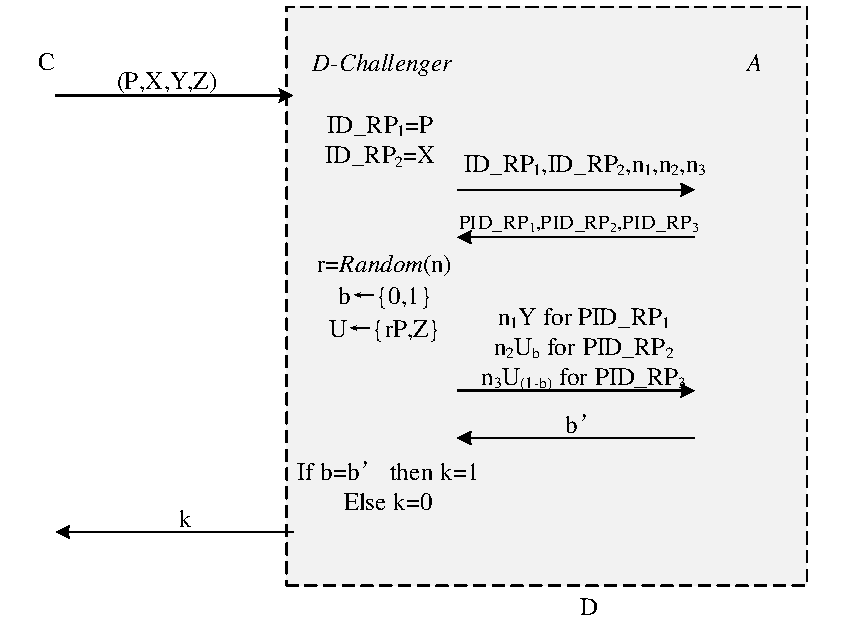
\includegraphics[width=0.97\linewidth]{fig/dalgorithm.pdf}
  \caption{The algorithm based on the RP-based identity linkage, to solve the ECDDH problem}
  \label{fig:dalgorithm}
\end{figure}

We define the RP-based identity linkage game $\mathcal{G}_r$:
after receiving $\mathfrak{L}$ and $L'$ from a challenger,
    the adversary outputs the result $s = 1$ if it decides $u' \in \{u_1, u_2, \cdots, u_v\}$ or $s = 0$ if $u'$ is randomly chosen in $\mathbb{Z}_n$.
The adversary's advantage in $\mathcal{G}_r$ is defined as $\mathbf{Adv}_{A}$.
%If the adversary is able to distinguish whether $u' \in \{u_1, u_2, \cdots, u_v\}$ or not,
%    the adversary will have non-negligible advantages in $\mathcal{G}_r$
%        and ${\rm Adv}_A$ is non-negligible.
Then,
\begin{align*}
&{\rm Pr}'_1={\rm Pr}\{\mathcal{G}_r(\mathfrak{L}, L'|ID_{U'} \in \{ID_{U_1}, ID_{U_2}, \cdots, ID_{U_v}\})=1\} \\
&{\rm Pr}'_2={\rm Pr}\{\mathcal{G}_r(\mathfrak{L}, L'|ID_{U'} \in \mathbb{Z}_n)=1\}\\
&{\mathbf{Adv}}_{A}=|{\rm Pr}'_1-{\rm Pr}'_2|
\end{align*}

We design a PPT algorithm $\mathcal{D}^*_r$ based on $\mathcal{G}_r$, shown in Figure \ref{fig:dalgorithm}, to solve the ECDDH problem.
The input is in the form of $(G$, $Q_1=[x]G$, $Q_2=[y]G$, $Q_3=[z]G)$.
On receiving the input, the challenger of $\mathcal{G}_r$ randomly chooses
 $\{u_1, u_2, \cdots, u_v\}$, $\{r_1, r_2, \cdots, r_c\}$, $\{t_{1, 1}, t_{1, 2}, \cdots, t_{v, c}\}$, and $t'$ in $\mathbb{Z}_n$.
Then the challenger constructs $\mathfrak{L}$ and $L'$ as below.
It firstly assigns $L_{i, j} = ([r_j]G, t_{i, j}, [u_ir_j]G)$, %$1\leq i \leq v$ and $1\leq j \leq c$,
    and randomly chooses $d \in [1, v]$ to
 replace $[u_d r_j]G$ with $[r_j]Q_1=[xr_j]G$ for $1\leq j \leq c$.
So $\mathfrak{L}=\left \{ \begin{matrix}
L_{1,1},&L_{1,2},&\cdots,&L_{1,c}\\
L_{2,1},& L_{2,2},&\cdots,&L_{2,c}\\
\cdots,&\cdots,&\cdots,&\cdots\\
([r_{1}]G, t_{d, 1}, [r_{1}]Q_1),&\cdots,&\cdots,&([r_{c}]G, t_{d, c}, [r_{c}]Q_1)\\
\cdots,&\cdots,&\cdots,&\cdots\\
L_{v,1},&L_{v,2},&\cdots,&L_{v,c}
\end{matrix}\right\}$.
%$L=$\{($[r_1]G$, $t_{1, 1}$, $[[u_1][r_1]G$), ($[r_2]G$, $t_{1, 2}$, $[u_1][r_2]G$), $\cdots$, ($[r_{\beta}]G$, $t_{\alpha, \beta}$, $[r_{\beta}]Q_1$), $\cdots$, ($[r_b]G$, $t_{a, b}$, $[u_a][r_b]G$)\}
%
The challenger assigns $L' = (Q_2, t', Q_3) = ([y]G, t', [z/y][y]G)$.
Finally,
    $\mathfrak{L}$ and $L'$ are sent to the adversary,
        and the output $s$ of $\mathcal{G}_r$ is output by the challenger.
According to the above construction of $\mathfrak{L}$ and $L'$,
    $x$ is actually inserted into $\mathfrak{L}$ as $u_d$
    and $z/y$ is assigned to $u'$.
So, if $z = xy$, then $z/y=x$ and $ID_{U'} \in \{ID_{U_1}, ID_{U_2}, \cdots, ID_{U_v}\}$;
    otherwise, $ID_{U'} \in \mathbb{Z}_n$.
Thus,
\begin{align*}
&{\rm Pr}_1={\rm Pr}\{\mathcal{D}^*_r(G, [x]G, [y]G, [xy]G)=1\}={\rm Pr}'_1 \\=&  {\rm Pr}\{\mathcal{G}_r(\mathfrak{L}, L'|ID_{U'} \in \{ID_{U_1}, ID_{U_2}, \cdots, ID_{U_v}\})=1\} \\
&{\rm Pr}_2={\rm Pr}\{\mathcal{D}^*_r(G, [x]G, [y]G, [z]G)=1\} ={\rm Pr}'_2 \\=&  {\rm Pr}\{\mathcal{G}_r(\mathfrak{L}, L'|ID_{U'} \in \mathbb{Z}_n)=1\}\\
&{\mathbf{Adv}}_{A}=|{\rm Pr}'_1-{\rm Pr}'_2|=|{\rm Pr}_1-{\rm Pr}_2|=\epsilon_{r}(k)
\end{align*}

The ECDDH assumption means that in $\mathcal{G}_r$ the adversary does not have advantages,
    i.e., cannot distinguish a user $U'$ chosen from \{${U_1}, {U_2}, \cdots, {U_v}$\}
        or randomly from the universal user set.
%    (indistinguishability of users to colluding RPs).
So the RP-based identity linkage is impossible. $\square$

